\documentclass[draftcls,onecolumn]{IEEEtran}

%% INCLUDING THE PREAMBLE
%%%%%%%%%%%%%%%%%%%%%%%%%%%%%%%%%%%%%%%%%%%%%%%%%%%%%%%%%%%%%%%%%%%%%%%%%%%
%                                                                         %
%                                 PREAMBLE                                %
%                                                                         %
%%%%%%%%%%%%%%%%%%%%%%%%%%%%%%%%%%%%%%%%%%%%%%%%%%%%%%%%%%%%%%%%%%%%%%%%%%%

%% PACKAGES
\usepackage[]{lineno}
%\linenumbers
\usepackage[usenames,dvipsnames]{xcolor}
\usepackage{microtype}
\usepackage[obeyDraft]{todonotes}
\usepackage{fancyvrb}
\VerbatimFootnotes
\usepackage{algorithmic}

%% GRAPHICS RELATED
\usepackage{graphicx}
\usepackage[outdir=./tmp/]{epstopdf}
\graphicspath{{../images/}{./}{./tmp/}}
\DeclareGraphicsExtensions{.eps, .pdf, .jpeg, .png,}

%% CPATION SETUP
\usepackage{float}
\usepackage{caption}
\usepackage{subcaption}
\captionsetup{belowskip=12pt,aboveskip=4pt}


%% BIBLIOGRAPHY
\bibliographystyle{ieeetr}

%% UNITS
\usepackage{siunitx}

%% EQUATIONS
\usepackage{amsmath}
%\numberwithin{equation}{section}

%% HYPERLINKS
\usepackage[debug]{hyperref}

%%%%%%%%%%%%%%%%%%%%%%%%%%%%%%%%%%%%%%%%%%%%%%%%%%%%%%%%%%%%%%%%%%%%%%%%%%%
%                                                                         %
%                             Listing Setup                               %
%                                                                         %
%%%%%%%%%%%%%%%%%%%%%%%%%%%%%%%%%%%%%%%%%%%%%%%%%%%%%%%%%%%%%%%%%%%%%%%%%%%
\usepackage{listings}
\lstset{ %
    language=C++,
    basicstyle=\footnotesize\ttfamily,
    numbers=left,
    numberstyle=\tiny\color{gray},
    stepnumber=2,
    numbersep=5pt,
    backgroundcolor=\color{white},
    showspaces=false,
    showstringspaces=false,
    showtabs=false,
    frame=single,
    rulecolor=\color{black},
    tabsize=2,
    breaklines=true,
    breakatwhitespace=false,
    title=\lstname,
    keywordstyle=\color{blue},
    commentstyle=\color{OliveGreen},
    stringstyle=\color{orange}
}
\DeclareCaptionFont{white}{\color{white}}
\DeclareCaptionFormat{listing}{\colorbox[cmyk]{0.43, 0.35, 0.35, 0.01}{\parbox{\dimexpr\textwidth-2\fboxsep\relax}{#1#2#3}}}
\captionsetup[lstlisting]{format=listing,labelfont=white,textfont=white,singlelinecheck=false,margin=0pt,font={bf,footnotesize}}
%\lstnewenvironment{code}[1][]%
%{ \noindent\minipage{\linewidth}
%	\lstset{#1}
%}
%{\endminipage}
%% USER COMMANDS
\usepackage{isotope}
\newcommand{\iso}{\isotope}
\newcommand{\figurewidth}{\textwidth}
\newcommand{\micron}{$\mu$m}



%%%%%%%%%%%%%%%%%%%%%%%%%%%%%%%%%%%%%%%%%%%%%%%%%%%%%%%%%%%%%%%%%%%%%%%%%%%
%                                                                         %
%                                Start of Document                        %
%                                                                         %
%%%%%%%%%%%%%%%%%%%%%%%%%%%%%%%%%%%%%%%%%%%%%%%%%%%%%%%%%%%%%%%%%%%%%%%%%%%
\begin{document}
\title{Comparison of Lithiated Glass, LiF:ZnS(Ag), Boron Loaded Plastic, and PEN Films}
\author{Matthew J. Urffer}
\date{\today}
\maketitle

% Tables of Contents, Figures, Tables
\tableofcontents
\listoffigures
\listoftables
%%%%%%%%%%%%%%%%%%%%%%%%%%%%%%%%%%%%%%%%%%%%%%%%%%%%%%%%%%%%%%%%%%%%%%%%%%%
%                                                                         %
%                              Start of Content                           %
%                                                                         %
%%%%%%%%%%%%%%%%%%%%%%%%%%%%%%%%%%%%%%%%%%%%%%%%%%%%%%%%%%%%%%%%%%%%%%%%%%%
\section{Introduction}

The potential application  of a material for use in a Radiation Portal Monitor (RPM) can be indicated by measurements of the detector's sensitivity to gammas and the detector's response to neutrons.
A detector material might be a possible replacement if the there exists a neutron response that can be differentiated from gammas for given sensitivity of gammas, namely \num{1E-6}.
A simple way to discriminate between gammas and neutrons is to have a pulse height discriminator for the gammas, above which there is only a 1 in a million chance that a gamma event will be classified as a neutron.
Under this framework, it is then possible to develop a mathematical lower level discriminator (MLLD) to function as this pulse height discriminator, and to then formulate the sensitivity requirement as the gamma intrinsic efficiency as a function of MLLD being less than \num{1E-6}.
Six detectors (three boron loaded plastic scintillators, one LiF:ZnS(Ag) doped screen, GS20, and an annealed composite PEN film\footnote{Sample was 12-Apr-2013, 25\% LiF, 70\% PEN, 5\% PPO-POPOP Annealed}) were then evaluated for their ability to perform in a RPM. 
The thickness of these detectors and mass of the absorber are shown in \autoref{tab:PhysicalProperties}.
\begin{table}[h]
\centering
\caption[Detector Physical Characteristics]{Physical characteristics of the detector.}
\label{tab:PhysicalProperties}
  \begin{tabular}{m{4cm}| m{2cm} m{2cm} m{2cm}}
  \toprule
    & Absorber & Thickness &  Mass Absorber (mg) \\
    \midrule
    EJ 254 2.5\% & \iso[10]{B} & 1/4" & 59.5 \\
    EJ 254 1\% & \iso[10]{B} & 1/4" & 23.8 \\
    EJ 254 5\% & \iso[10]{B} & 3/4 & 356.1 \\
    EJ 425 HD2-PE & \iso[6]{Li} & \SI{0.1}{\mm} & 17.5 \\
    GS20 & \iso[6]{LI} & \SI{2}{\mm} & 155 \\
    Annealed Composite PEN Film & \iso[6]{Li} & $\approx$ \SI{250}{\um} & 28.1 \\
    \bottomrule
  \end{tabular}
\end{table}

\subsection{Previous Work}

Work by Guerard (published slides) has published slides of the performance of GS20 and a LiF:ZnS film (\autoref{fig:GuerardLightYield}).
It should be noted for the start that Guerard's measurement is not the same as ours - the neutron source is unknown, as well is the supplier of the LiF:ZnS film (and thickness). 
In addition, the thickness of GS20 reported by Guerard is \SI{0.5}{\mm} while the GS20 in the detection lab is \SI{2}{\mm}.
\begin{figure}
  \centering
  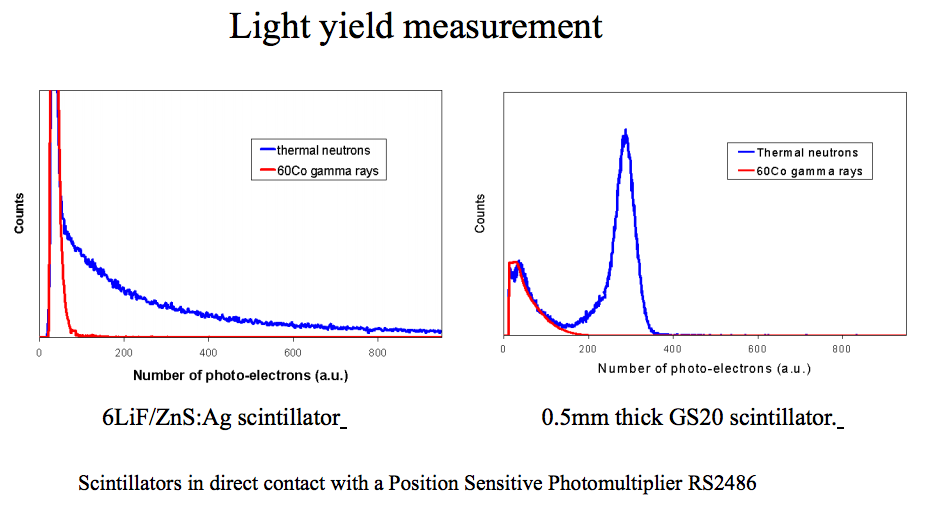
\includegraphics[width=\textwidth]{Guerard_LightYieldMeasurement}
  \caption[Measured Light Yield (Guerard)]{Light yield as measured by Guerard. The GS20 measurement has a lower gamma performance than as measured, and the LiF:ZnS does not have the same shape as we measured}
	\label{fig:GuerardLightYield}
\end{figure}
The following figure, \autoref{fig:GuerardIntEff}, shows the neutron detection efficiency and sensitivity to \iso[60]{Co} rays.
For a sensitivity of \num{10E-6} the LiF:ZnS film is reported to have a neutron detection efficiency of 60\%, while the \SI{1}{\mm} GS20 has a reported neutron detection efficiency of 55\%.
\begin{figure}
  \centering
  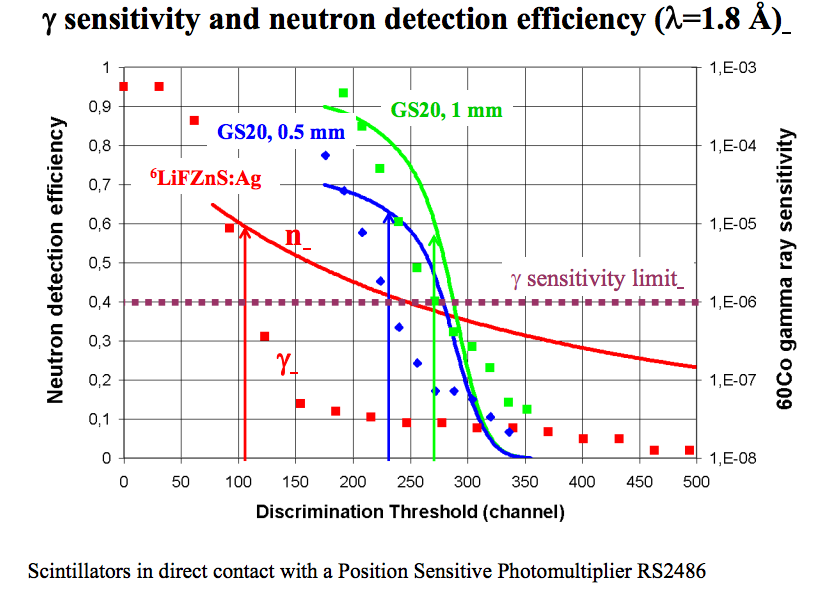
\includegraphics[width=\textwidth]{Guerard_IntEff_NCr}
  \caption[Intrinsic Efficiency (Geurard)]{Intrinsic Efficiency of LiF:ZnS and GS20 from Guerard.  The gamma intrinsic efficiency is shown in the solid squares (right axis), while the lines show the neutron efficiency (left axis). The values reported here are much higher than the values reported in this report.}
	\label{fig:GuerardIntEff}
\end{figure}

\section{Methods}
The detectors were measured between April 28, 2013 and May 2, 2013 in the radiation characterization laboratory.
The neutron performance was determined a \iso[252]{Cf} irridiator previously described, and the gamma source was the \iso[60]{Co} irridiator.
Due to the wide range of light output of these films it was necessary to use a two voltages (\SI{1000}{\volt} and \SI{1180}{\volt}) in order to capture the entire spectra.
However, a measurement of the GS20 peak in the lead well was always recorded which then allowed the spectra to be tied together based on this feature, as shown in \autoref{eqn:SettingScale}.
\begin{align}
  \label{eqn:SettingScale}
  \text{Channel Feature at Setting A} = \frac{\text{Channel GS20 Peak at Setting A}}{\text{Channel S20 Peak at Setting B}} \;\; \left( \text{Channel Feature at Setting B}\right)
\end{align}
The count rates are not scaled for gain and voltage settings, as they should remain constant as long as counts are not pushed below the lower level discriminator or cause roll-off.
\subsection{Neutron Performance above Gamma Discriminator}
An accurate measure of the neutron performance above the pulse height discriminator is essential for the comparison between detector materials.
In \autoref{fig:GammaMLLDIntEff} it is shown that the location of the MLLD is a pretty stable measurement.
\begin{figure}
  \centering
  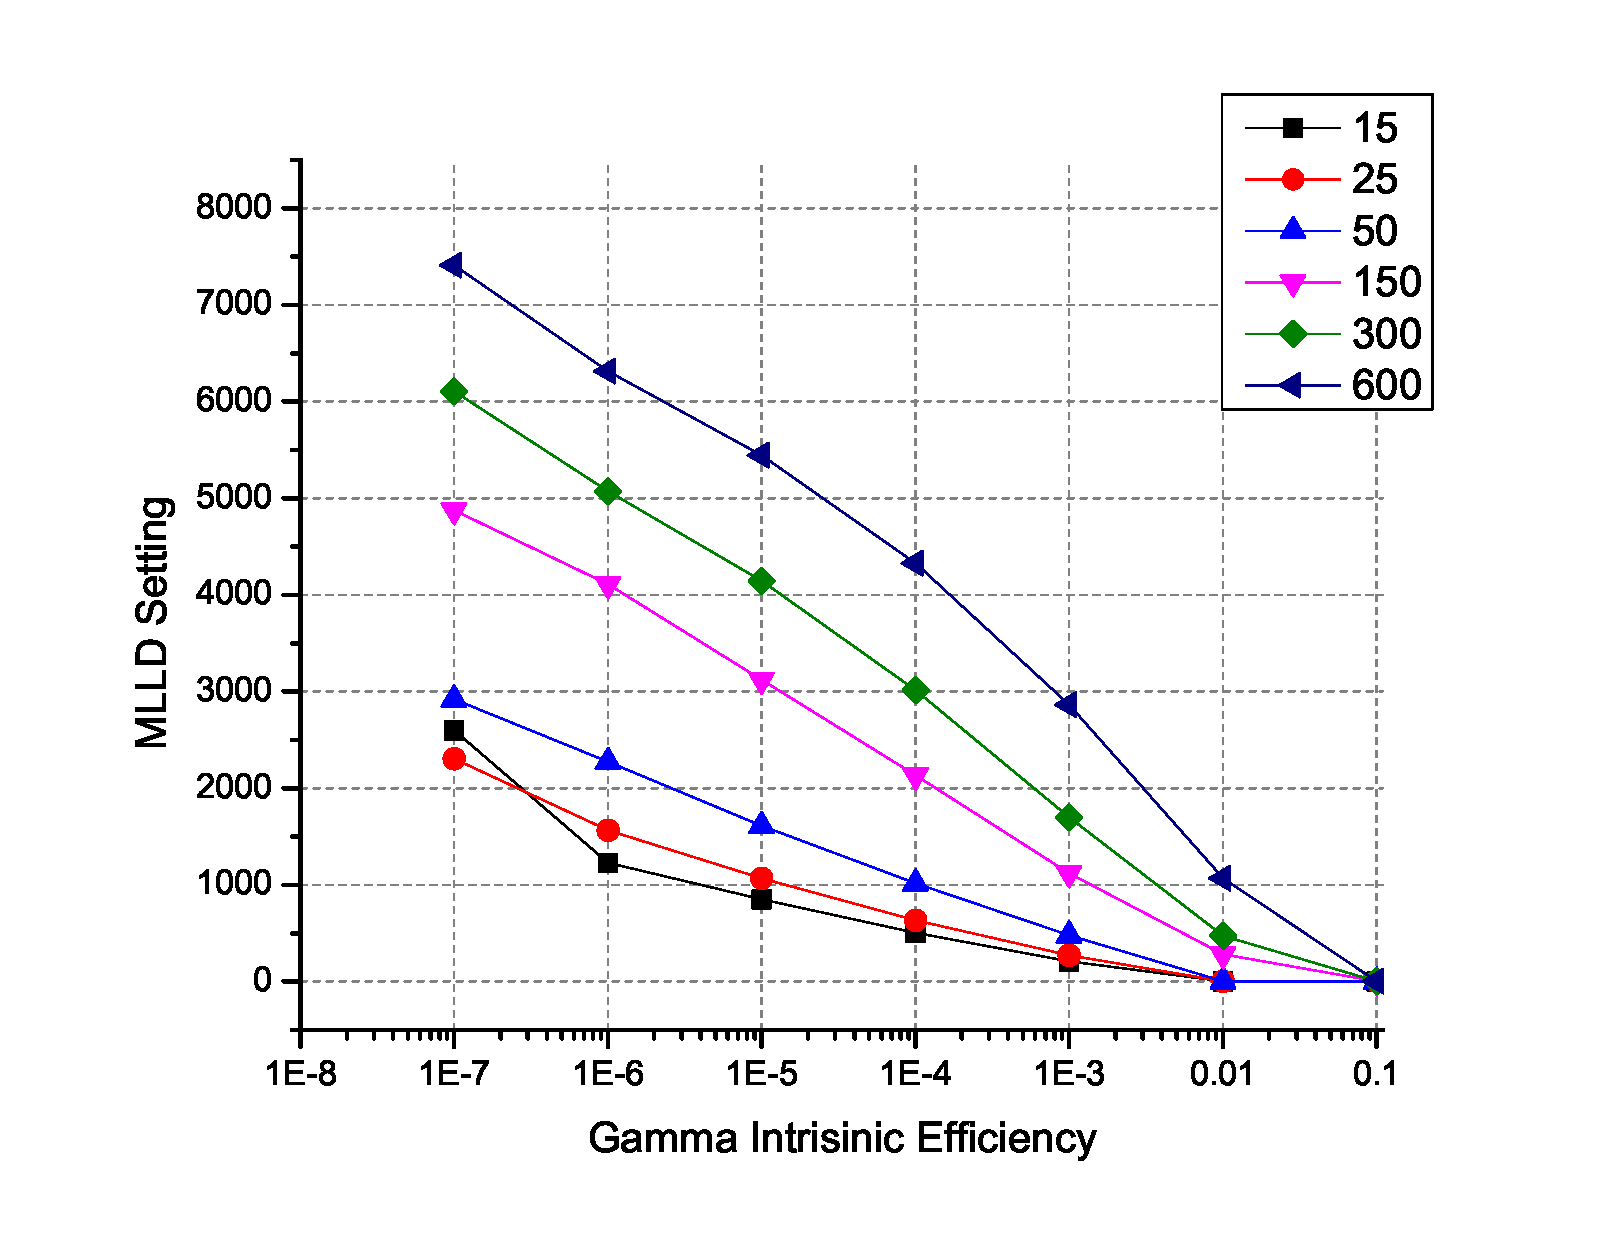
\includegraphics[width=\textwidth]{PS_IntEffMLLD_LiF}
  \caption[Stability of Lower Level Discriminator]{The mathematical lower level discriminator (MLLD) as a function of intrinsic effigies for 10\% PS films of various thickness. The linear nature suggest that the determination of the MLLD is repeatable.}
  \label{fig:GammaMLLDIntEff}
\end{figure}
However, in previous work which focused on using the fraction of neutron counts above the MLLD it was observed that the fraction (as it is normalized by the entire count rate) is very susceptible to noise in the low energy channels.
Therefore, after extensive studies using the polystyrene matrix a more stable measure was found by simply integrating the counts above in the neutron spectra above the MLLD and then normalizing by the mass of neutron absorber in the samples \autoref{eqn:CountRateAbovePerMass}.
While this method does not have the errors associated with summing over the low channels, it does require an accurate measure of the mass of \iso[6]{Li} in the sample.
\begin{align}
\label{eqn:CountRateAbovePerMass}
\eta = \frac{\int_{\text{MLLD}}^\infty p(x)dx}{\text{Neutron Absorber Mass}}
\end{align}

\section{Results}
The following figures, \autoref{fig:Co60Spectra} and \autoref{fig:PbWellSpectra}, show the measured spectra of the detectors to neutrons and gammas.
It is clear that the EJ-254 films will have poor performance because of their large gamma response.
The EJ-426 has the lowest response of them all, and it is not clear if the tail of the spectra is actually counts or background.
In the neutron spectra it was decided to only plot the performance of the best EJ-254 (though \autoref{fig:EJ254Perf} display the performance of all EJ-254 films).
It is observed that the LiF:ZnS(Ag) is much brighter than the other films, and it is noted that the annealed composite PEN has a high light output than the commercial EJ-254 based on the peak location.
\begin{figure}
  \centering
  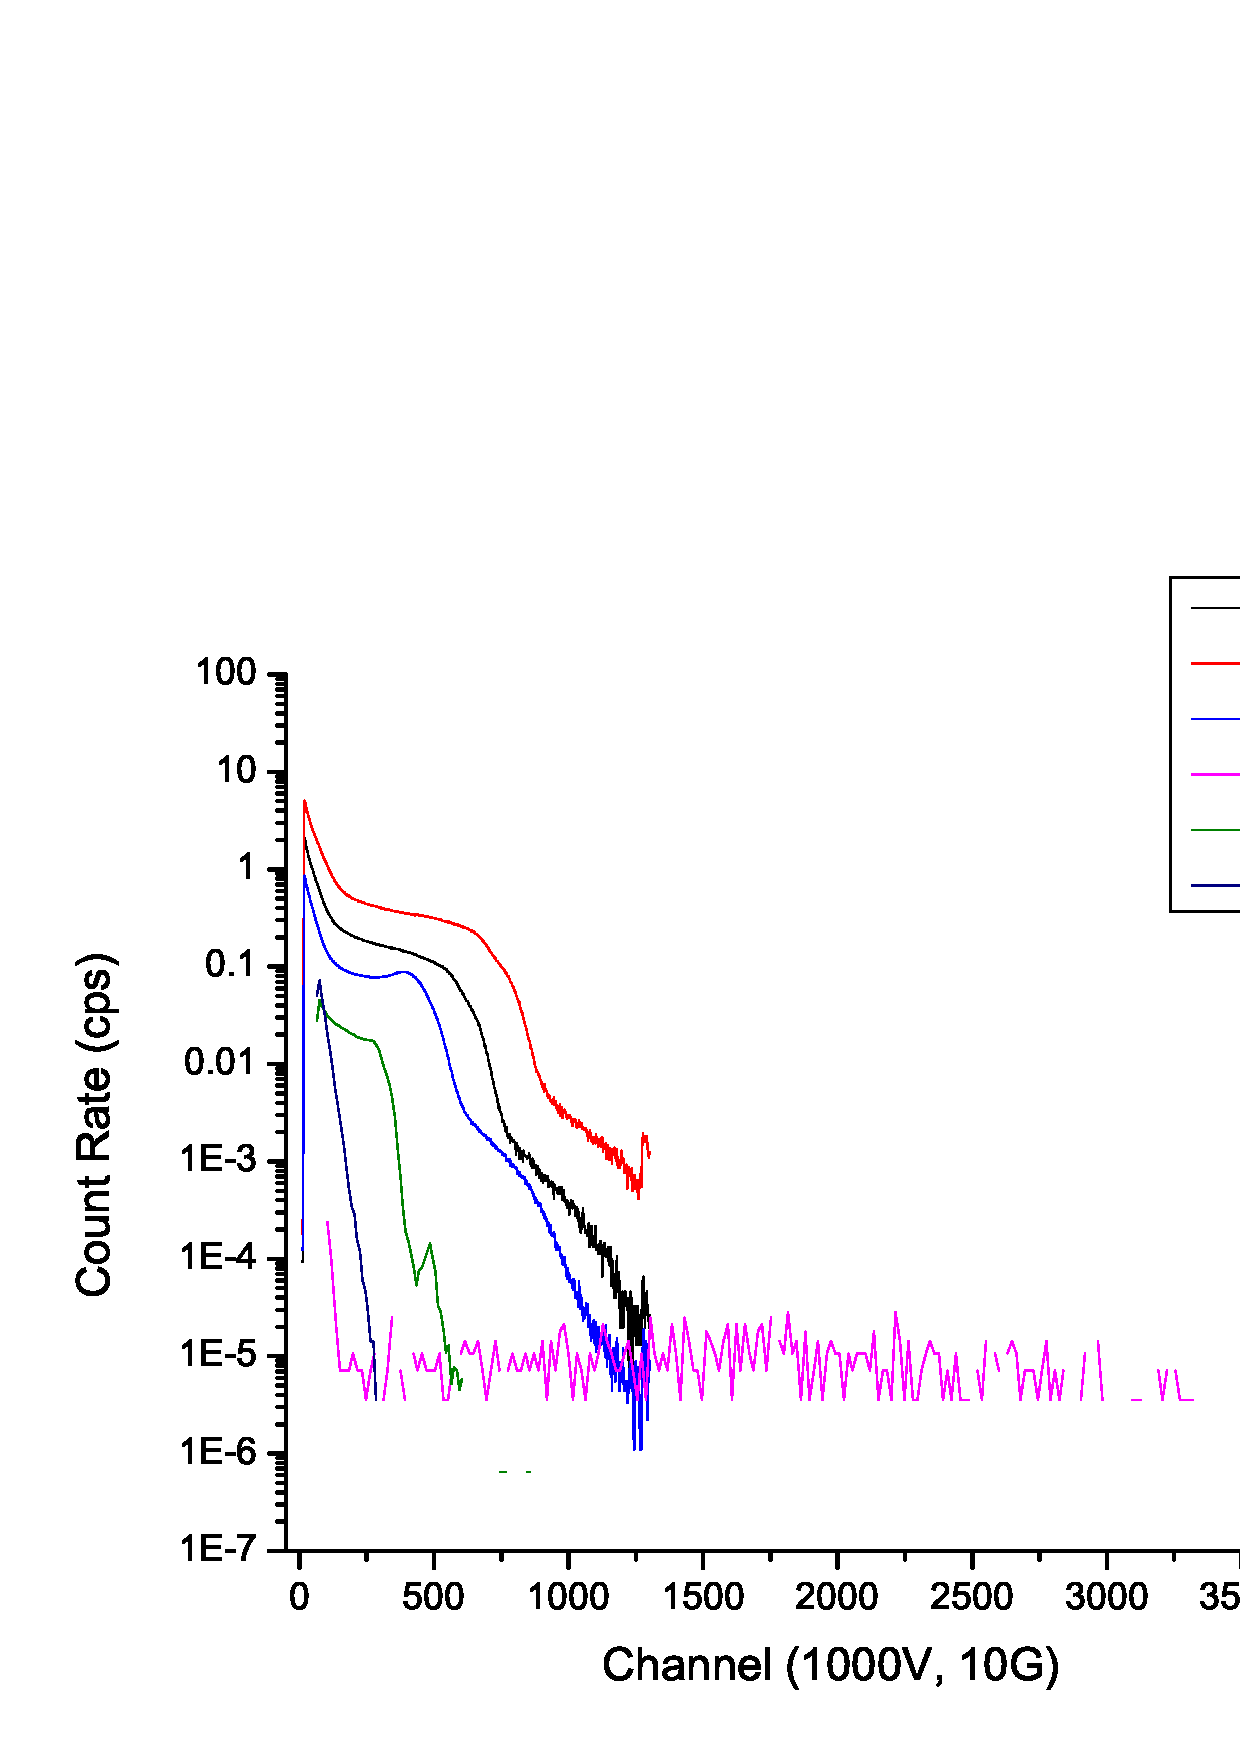
\includegraphics[width=\textwidth]{SampleComparions_Co60Spectra}
  \caption[Gamma Response of Measured Detectors]{Gamma Response from \iso[60]{Co} source of measured detectors.}
  \label{fig:Co60Spectra}
\end{figure}
\begin{figure}
  \centering
  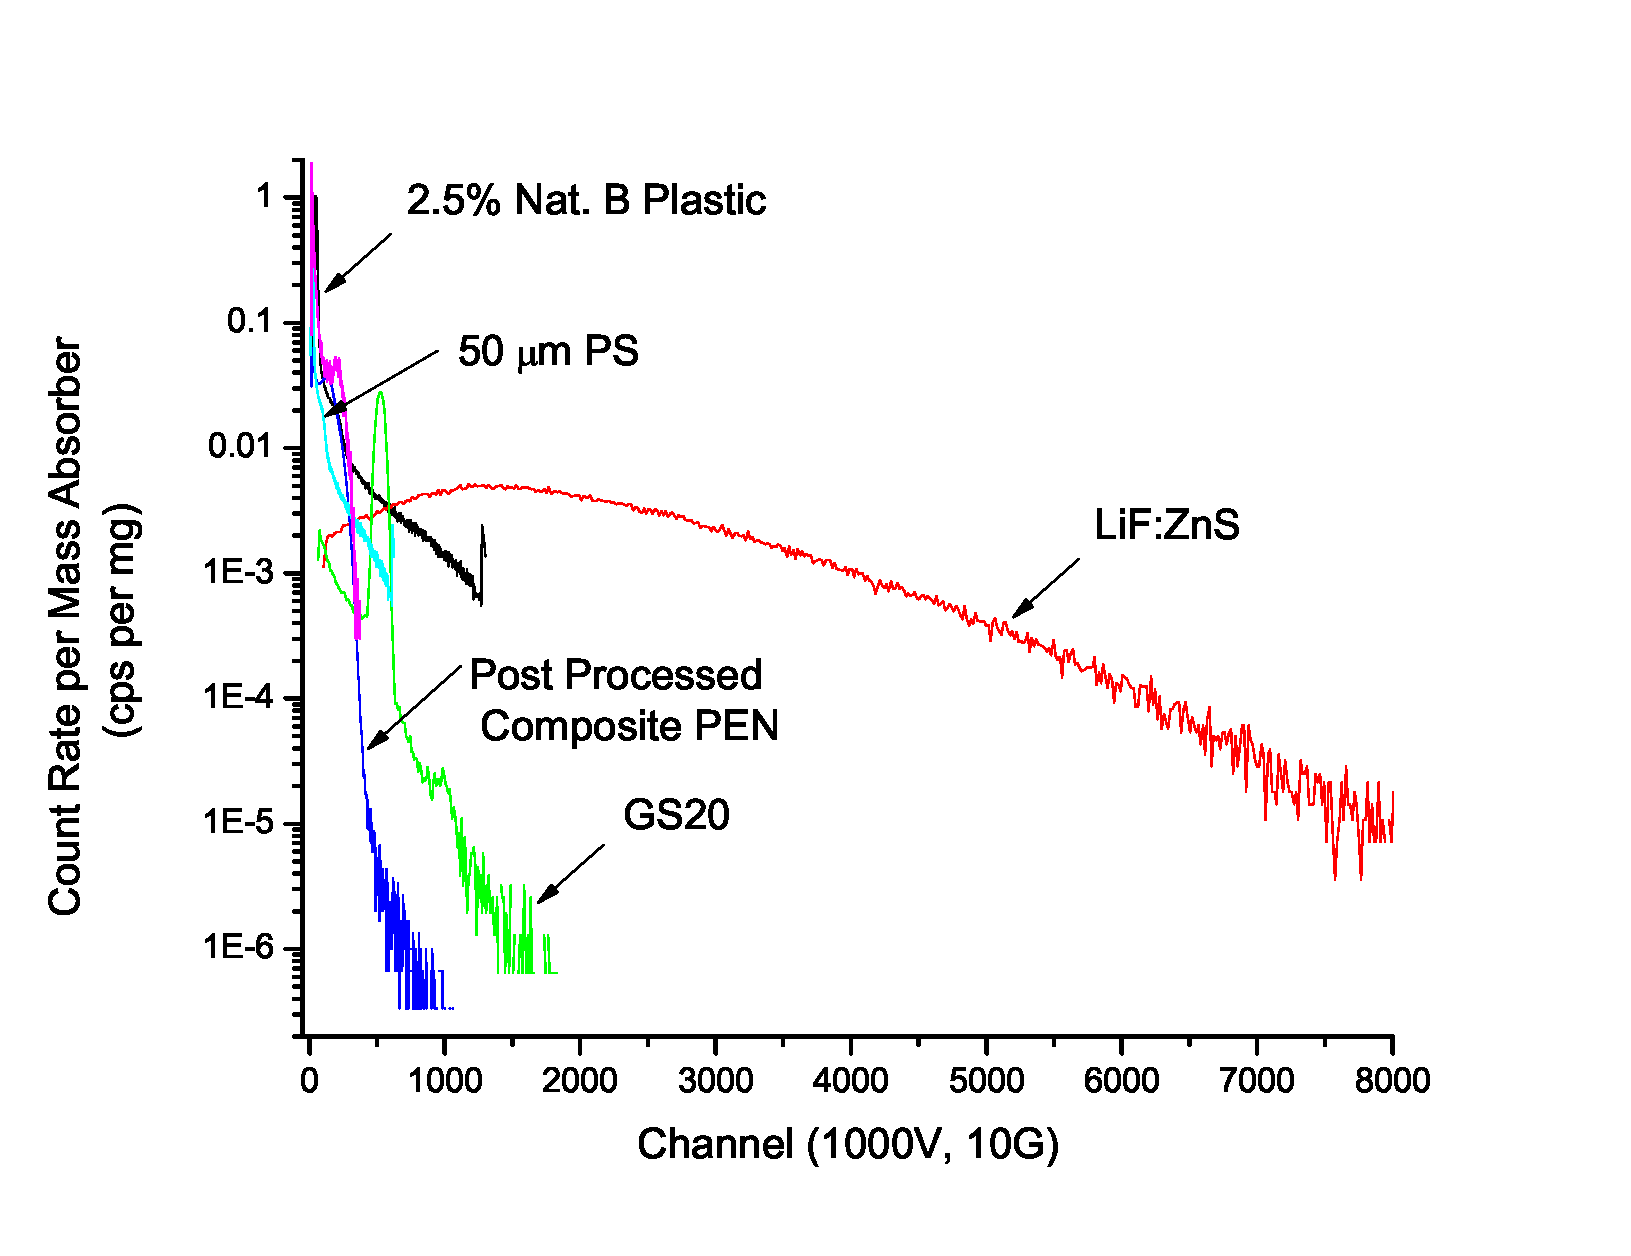
\includegraphics[width=\textwidth]{SampleComparison_PbCRperMg}
  \caption[Neutron Response of Measured Detectors]{Neutron Response (lead well) of the measured detectors. The count rate has been normalized by the mass of neutron absorber in the detector.}
  \label{fig:PbWellSpectra}
\end{figure}
The average channel number of the neutron and gamma spectra of each detector was calculated and are presented in \autoref{tab:AvgChNG}.
The average was computed for the neutrons in the thermal well to avoid the low energy channels from shifting the spectra away from any peak location.
It should be noted that for the EJ-254 the low channel number average is correct; the peak at this feature was identified as the neutron spectra.
\begin{table}
  \centering
  \caption[Average Channel Number of Gamma and Neutron Spectra]{Average channel number of gamma and the thermal neutron spectra .  The channel averages are scaled to 1,000V, 10G. The light yields are scaled to GS20 having 3,800 photons per MeV, and 6,250 photons per Neutron.}
  \label{tab:AvgChNG}
  \begin{tabular}{c| c c |c c}
    \toprule
        &\multicolumn{2}{|c|}{Gamma}&\multicolumn{2}{|c}{Neutron}\\
        & Average Channel& Photons per MeV & Average Neutron Channel & Photons per Neutron\\
    \midrule
    EJ 254 2.5\%, 1/4"&	183.41	&	4034.25	&	54.06	&	644.68	\\
    EJ 254 1\%, 1/4"&	216.25	&	4756.47	&	65.04	&	775.59	\\
    EJ 254 5\%, 3/4"&	176.49	&	3881.87	&	39.56	&	471.80	\\
    EJ 426 HD2&	1636.53	&	35995.87	&	2018.46	&	24070.77	\\
    GS20 &	172.76	&	3800.00	&	524.10	&	6250.00	\\
    Annealed Composite PEN&	87.63	&	1927.48	&	160.07	&	1908.87	\\
    \bottomrule
  \end{tabular}
\end{table}
The count rates of the detectors are presented in \autoref{tab:CountRate} for both the thermal component as well as only in the lead well spectra.
\begin{table}
\centering
  \caption[Detector Count Rate]{Count rate of the detectors in the thermal spectra as well as the lead well spectra.  The final two columns are normalize by the mass of the absorber in the material.}
  \label{tab:CountRate}
  \begin{tabular}{c | c c| c c}
  \toprule
    &\multicolumn{2}{|c|}{Count Rate (cps)}&\multicolumn{2}{|c}{Count Rate per Mass Absorber (cps per mg)} \\
    & Thermal Neutrons &Lead Well & Thermal Neutrons & Lead Well\\
  \midrule
  EJ 254 2.5\%, 1/4"&	1104	&	1869	&	18.5	&	31.4	\\
  EJ 254 1\%, 1/4"&	447	&	1130	&	18.8	&	47.5	\\
  EJ 254 5\%, 3/4"&	1417	&	3415	&	3.98	&	9.59	\\
  EJ 42 6 HD2 \SI{0.1}{\mm}&	224	&	234	&	12.8	&	13.4	\\
  GS20 \SI{2}{\mm}&	328	&	412	&	2.12	&	2.66	\\
  Annealed Composite PEN $\approx$ \SI{250}{\um}&	176	&	195	&	6.26	&	6.93	\\
  \bottomrule
  \end{tabular}
\end{table}
\autoref{tab:DiscrimPreformance} shows the discrimination performance of the tested detectors, while \autoref{fig:DiscrimPerformance} plots the intrinsic efficiency (sensitivity) along with the neutron count rate, normalized by the absorber mass.
\begin{table}
  \centering
  \caption[Discrimination Performance]{Discrimination performance of the measured films}
  \label{tab:DiscrimPreformance}
  \begin{tabular}{c | c c}
    \toprule
    &	MLLD Location	&	Count Rate above per Absorber Mass (cps per mg)	\\
    \midrule
    EJ 254, 2.5\% B, 1/4"	&	1280	&	0.20	\\
    EJ 254, 1\% B, 1/4"	&	1300	&	0.05	\\
    EJ 254, 5\% B, 3/4"	&	1290		&	0.03	\\
    EJ 426 HD2, \SI{0.1}{\mm}&	3308		&	1.97	\\
    GS20, \SI{2}{\mm}	&	557		&	0.56	\\
    Annealed Composite PEN, $\approx$ \SI{250}{\um}	&	209	&	1.96	\\
    \bottomrule
\end{tabular}
\end{table}
\begin{figure}
  \centering
  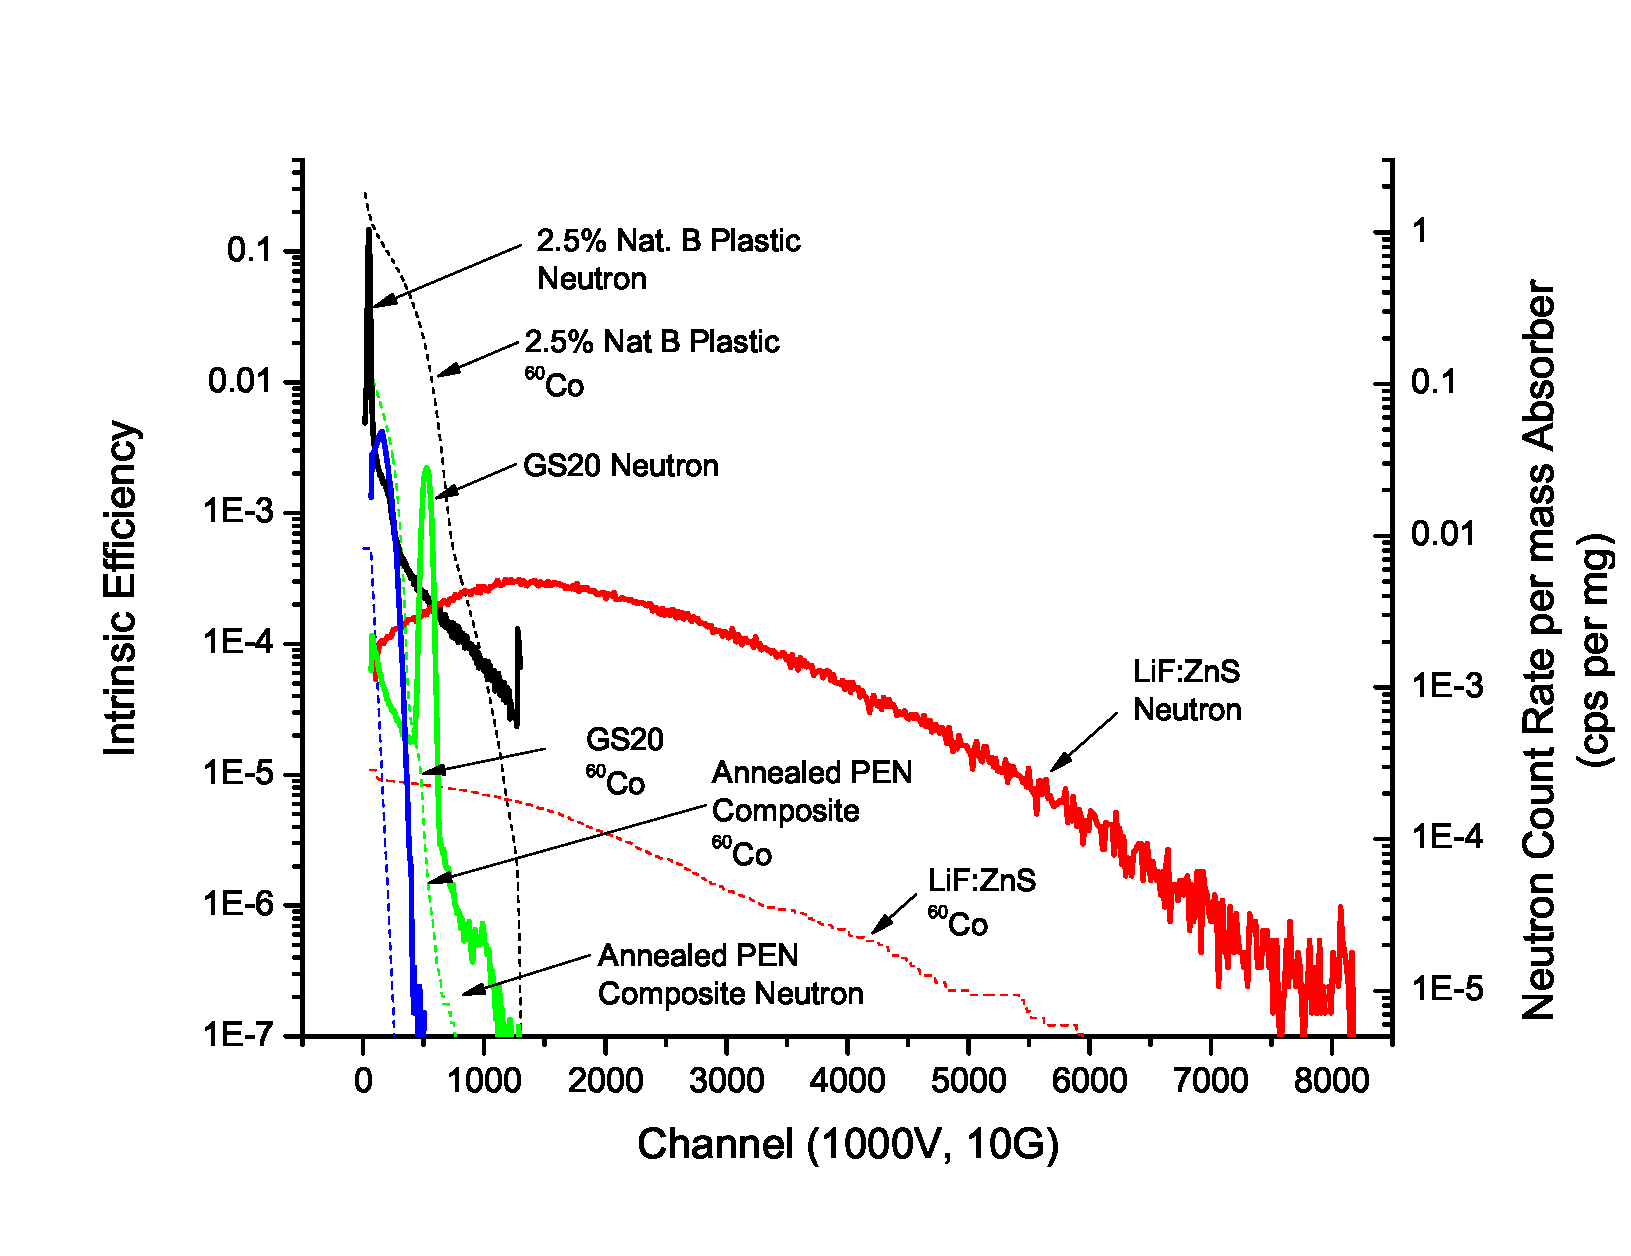
\includegraphics[width=\textwidth]{SampleComparison_IntEff_CR}
  \caption[Gamma Sensitivity and Neutron Response of Measured Detectors]{Gamma sensitivity (left axis) and neutron performance (right axis) of measured detectors.  The neutron count rate above the gamma pulse height discriminator may be found by noting where the intrinsic efficiency crosses \num{1E-6} and then integrating the neutron spectra above it. The neutron spectra are from the lead well, and are normalized by the mass of absorber.}
  \label{fig:DiscrimPerformance}
\end{figure}

\subsection{Individual Detector Performance}
After determining the general detector the performance of an individual detector is shown such that features are more visible.
\begin{figure}
  \centering
  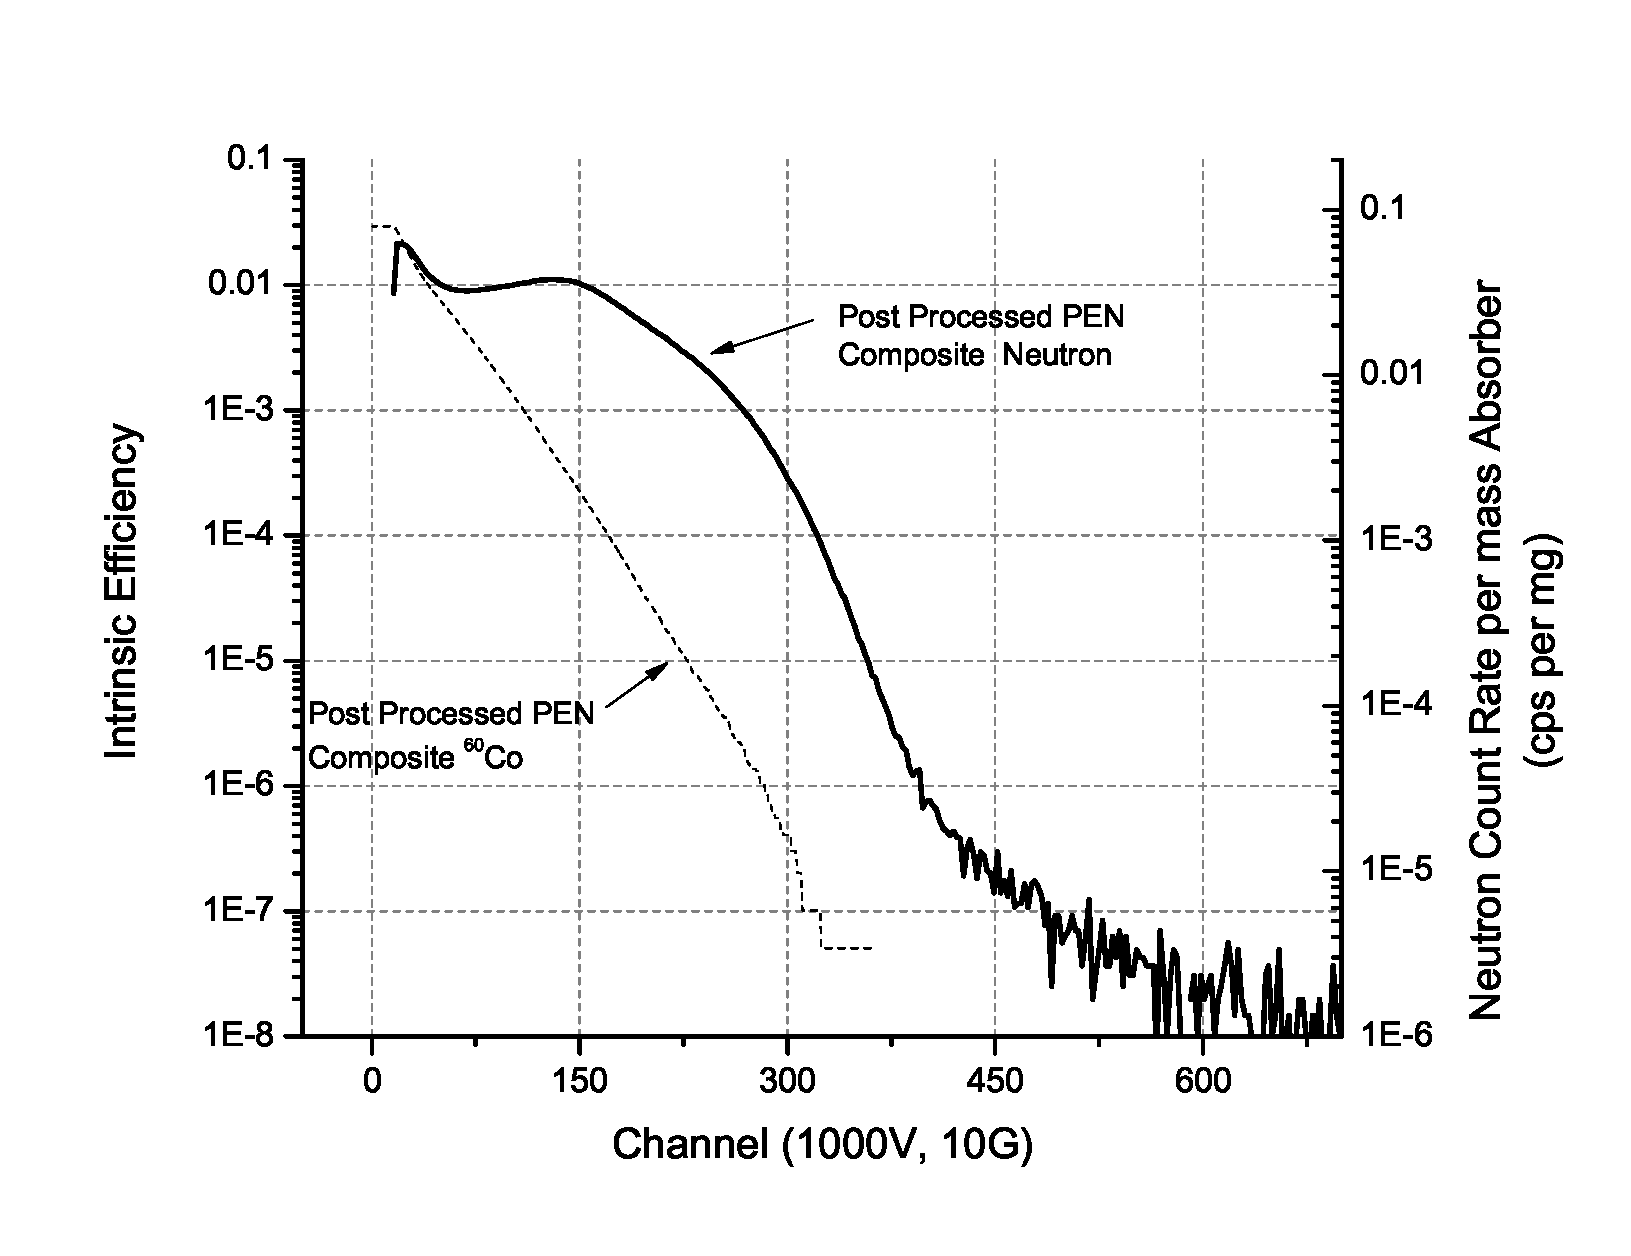
\includegraphics[width=\textwidth]{SC_ACPEN_IntEff_CR}
  \caption[Annealed Composite PEN Performance]{Performance of an Annealed Composite PEN Film (12 April Sample).}
  \label{fig:ACPENPreformance}
\end{figure}
\begin{figure}
  \centering
  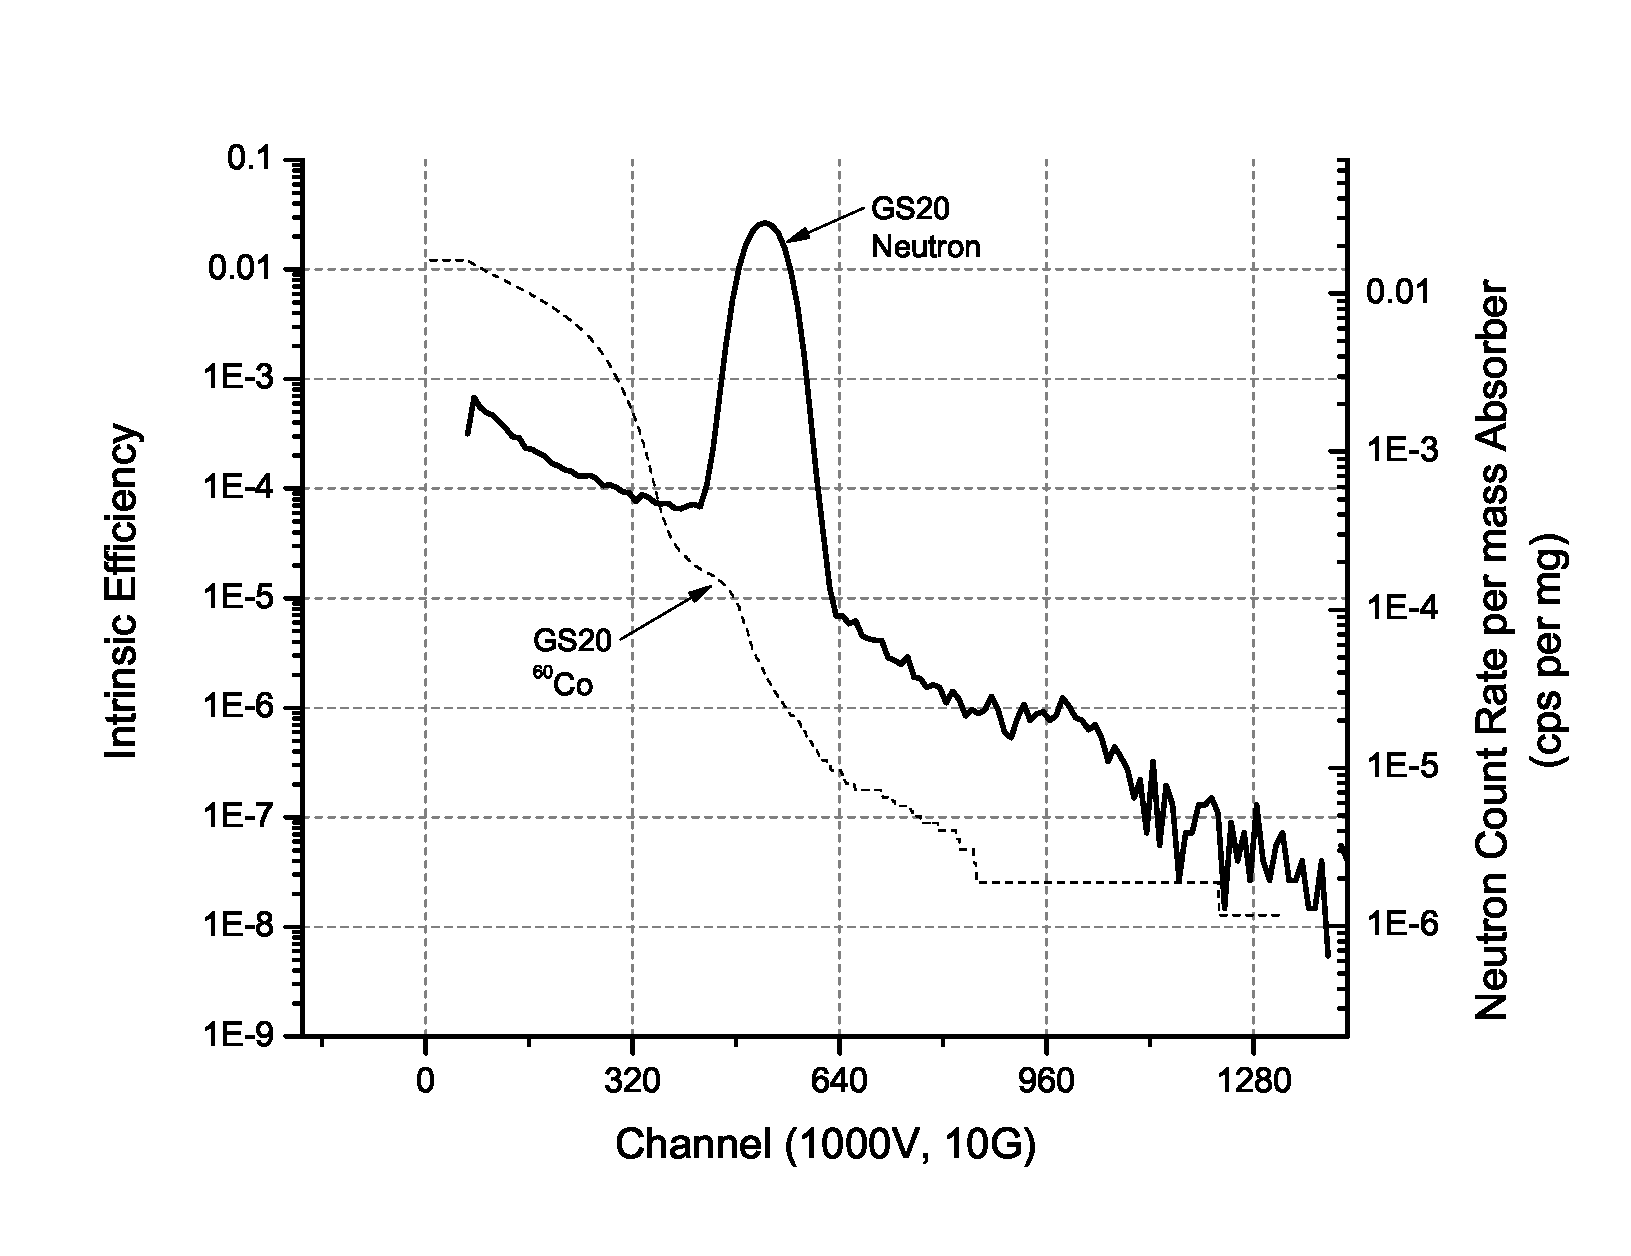
\includegraphics[width=\textwidth]{SC_GS20_IntEff_CR}
  \caption[GS20 Performance]{Performance of \SI{2}{\mm} GS20.  It should be noted that there is significant self shielding in GS20, and that due to the gamma sensitivity catching the tail of the neutron peak the count rate above the gamma pulse height discriminator has the most variation of the samples measured.}
  \label{fig:GS20Preformance}
\end{figure}
\begin{figure}
  \centering
  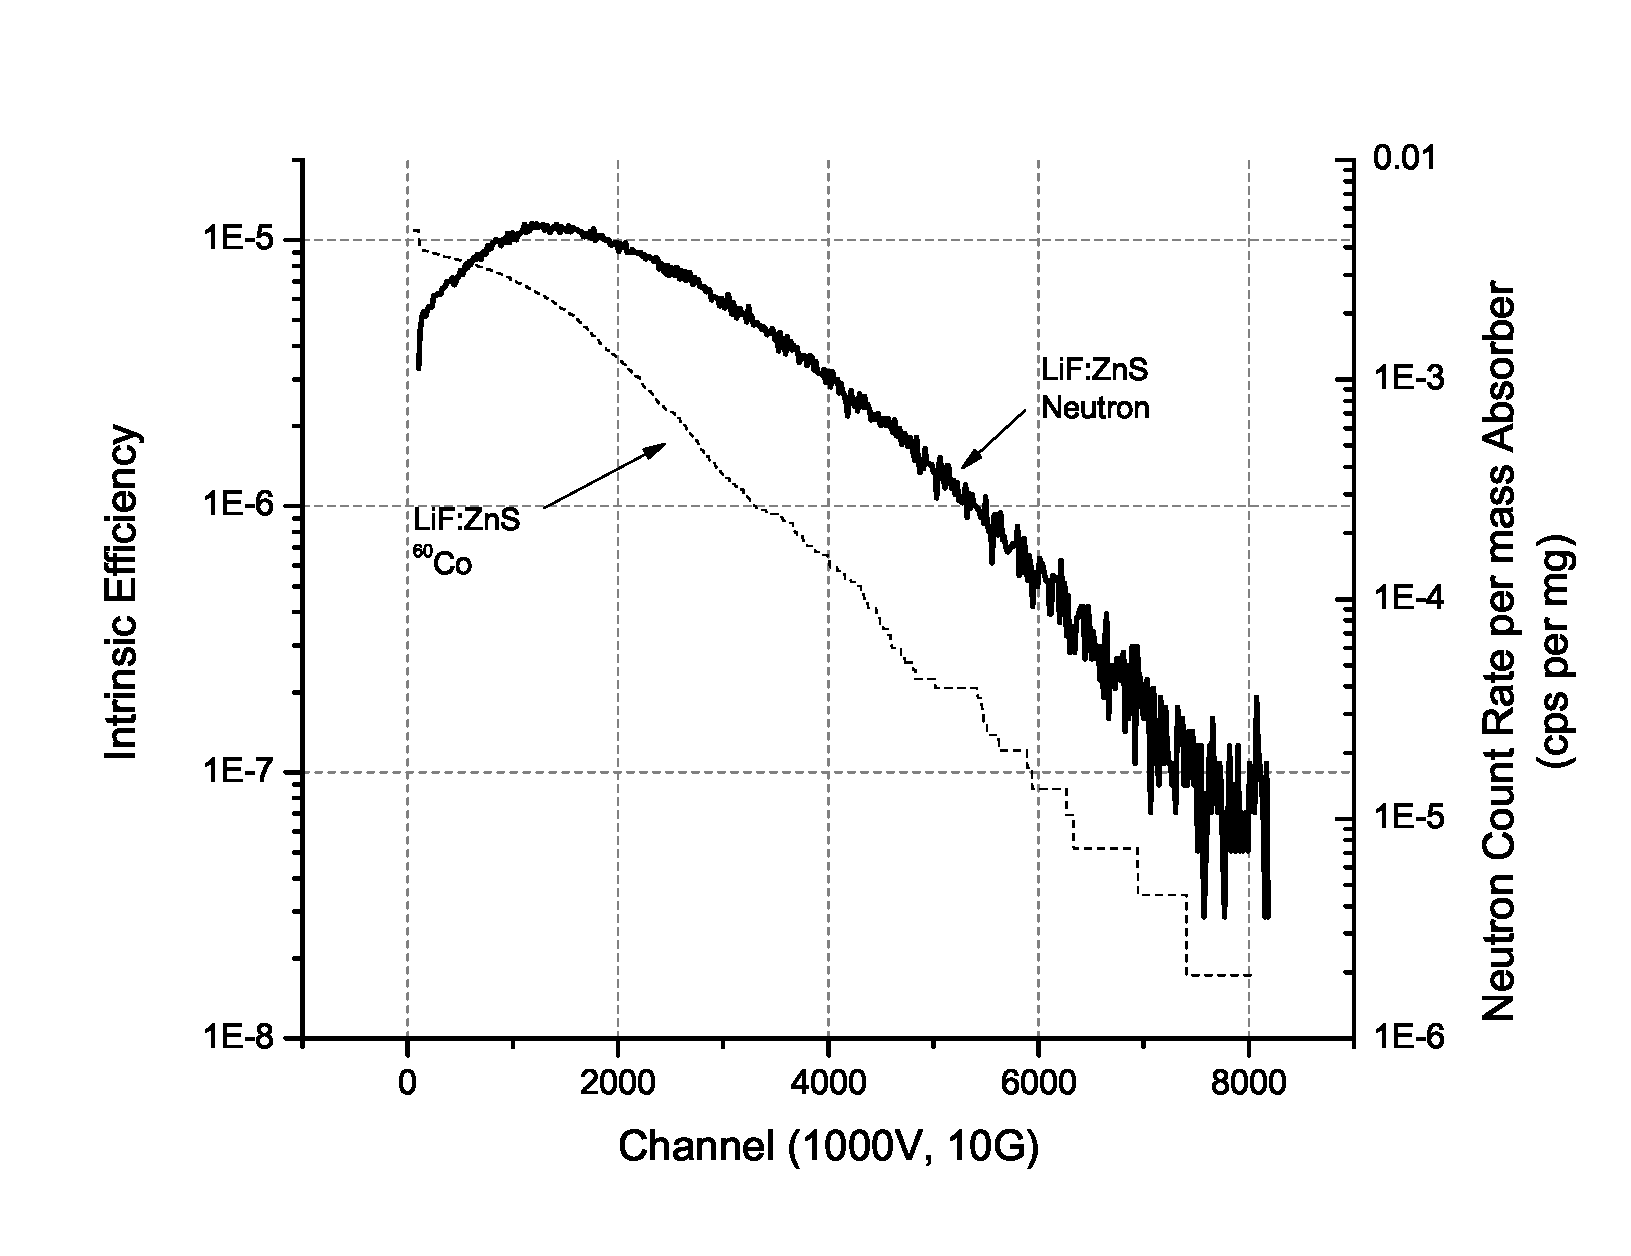
\includegraphics[width=\textwidth]{SC_EJ426_IntEff_CR}
  \caption[EJ 426 Preformance]{Preformance of EJ-426 HD2 (LiF:ZnS(Ag)) sheet.  This is the brightest scintillator tested, with the lowest gamma sensitivity.}
  \label{fig:EJ254Perf}
\end{figure}
\begin{figure}
  \centering
  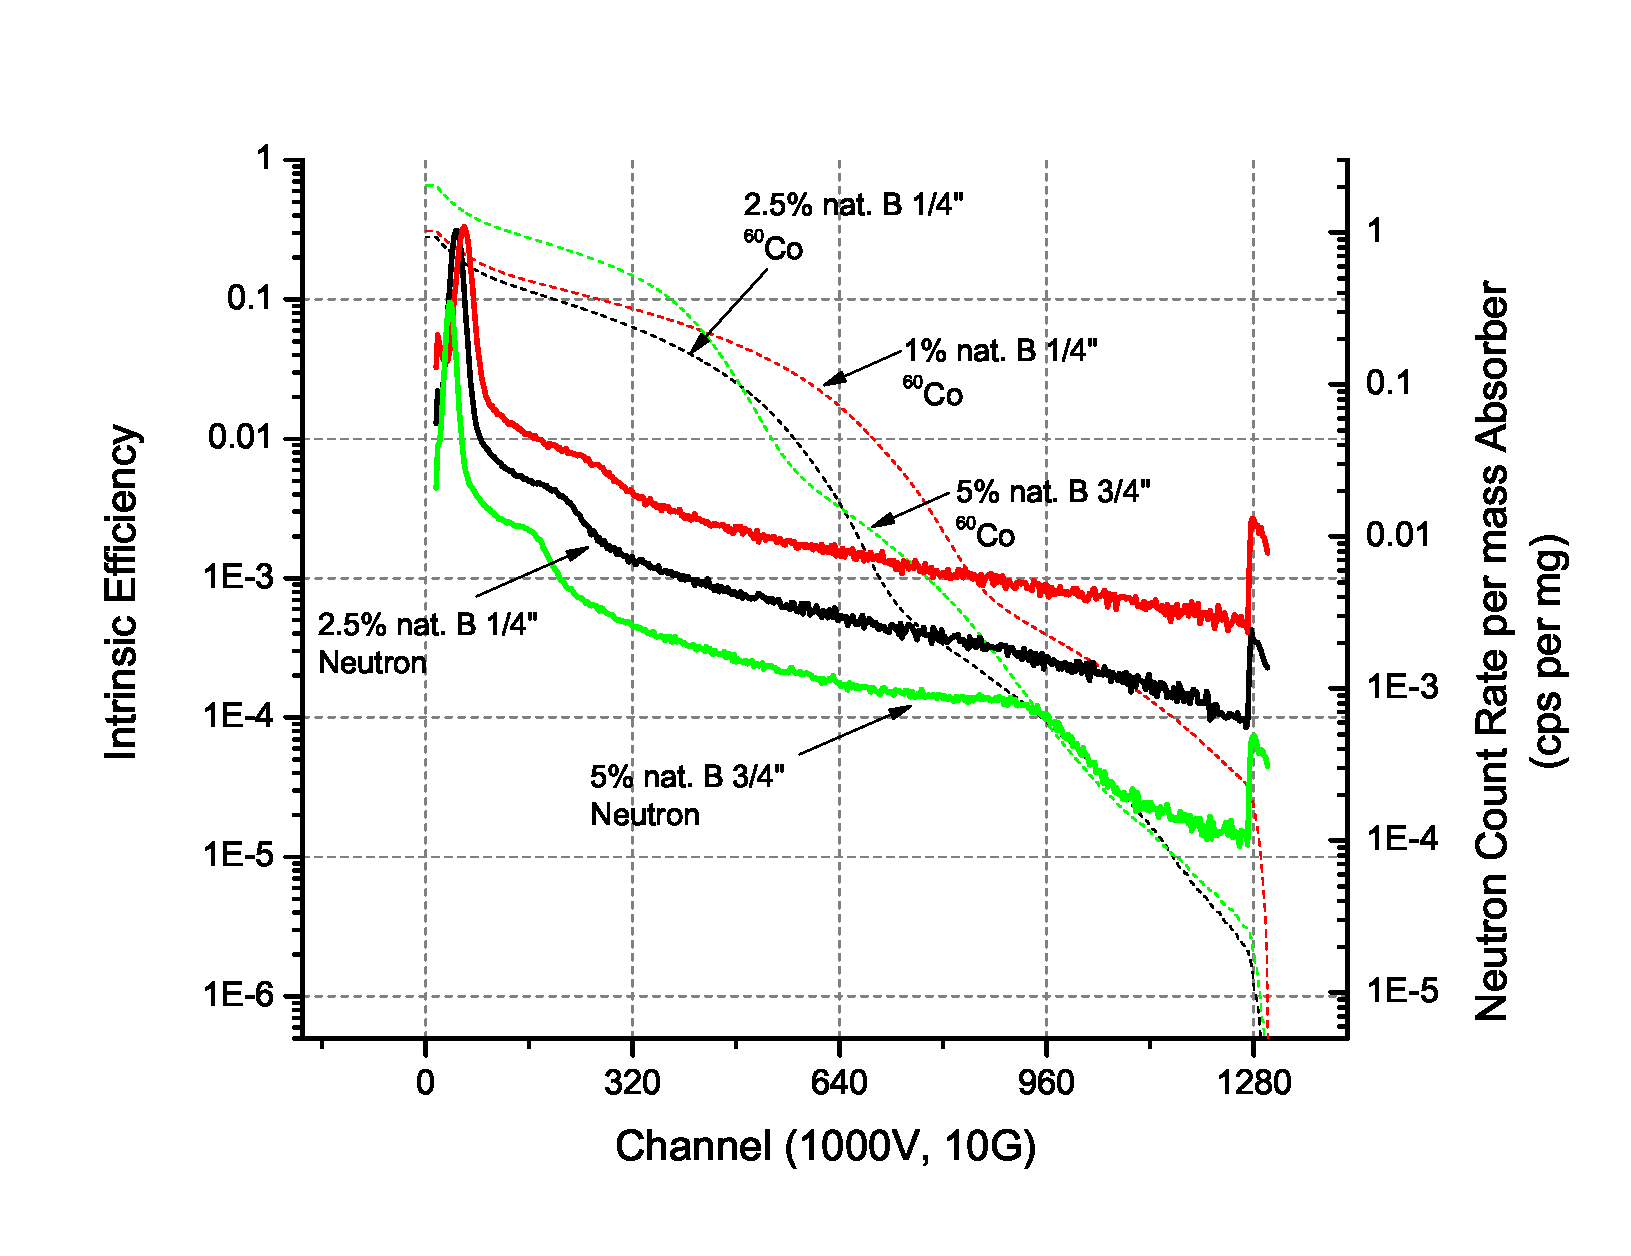
\includegraphics[width=\textwidth]{SC_EJ254_IntEff_CR}
  \caption[EJ 254 Preformance]{Preformance of EJ-254}
  \label{fig:EJ254Preformance}
\end{figure}
It is apparent that the EJ-254 is not a suitable candidate for replacement detector material in an RPM using a pulse height discriminator.
The reasons for this are twofold: 1) the detector is very thick which increases the probability of a gamma interaction as well as the probability that the interaction will deposit a majority of its energy and 2) \iso[10]{B} has a much lower Q-value (\SI{2.78}{\MeV} compared to \SI{4.78}{\MeV}) and a large pulse height deficit.
However, the material is optically transparent and due to \iso[10]{B}'s large thermal perhaps a thin sheet of EJ-254 might make a suitable detector material.
\subsection{Agreement to Previous Results}
It is observed from \autoref{fig:GuerardIntEff} that the neutron spectra has the same endpoint while the gamma sensitivity increases with thickness.
Assuming a linear increase in the gamma sensitivity with thickness and apply a linear extrapolation, a \SI{2}{\mm} would then be expected to have a discrimination threshold for \num{1E-6} at 350 channels, at which point the neutron detection efficiency is less than a few percent.
This agrees with previous measurements of the fraction of counts above the MLLD for GS20, which tend to be about 4\%.

\section{Conclusions}
Six detectors were tested for their ability to serve as possible replacement detectors in the RPM8.
Of the six tested, all but the EJ-254 (a boron loaded plastic scintillator at least 1/4" thick) could serve as possible replacements based on having neutron counts above a gamma rejection of one in a million.
The EJ-254 might be a possible replacement if it was made thinner to limit the gamma interactions and energy deposition when an interaction occurs.
\section{Appendix}
The EJ-254, EJ-426, GS20, and annealed composite PEN spectra data contained in this report may be found at \verb+Dropbox/SpectraFiles/(0)_2013_Data/SampleComparison_28Apr2013+.
These files were measured from April 28, 2013 to May 2, 2013, with the voltage, gains and count times recorded in the lab notebook. 
Of the spectra recorded, it was decided to go with Trial 1 when duplicate trials were made.
Corresponding hand calculations can be found on pages 104-106 of Matthew Urffer's 2nd lab book.

\end{document}
